% Soutenance M2 ISF — Agrégation byzantine-résiliente : la librairie Krum
% Auteur : Arthur Danjou — CMAP, École Polytechnique
% Build : latexmk -pdf slides.tex (moteur pdflatex, sans biber)
% Durée : 29 minutes de contenu et une minute de marge.
% Les commentaires MIN indiquent les repères de l'horloge.
\documentclass[aspectratio=169, 10pt]{beamer}

% --- Langue et fontes ---
\usepackage[utf8]{inputenc}
\usepackage[T1]{fontenc}
\usepackage[french]{babel}
\usepackage{lmodern}

% --- Maths ---
\usepackage{amsmath, amssymb}

% --- Présentation institutionnelle ---
\usetheme{default}
\setbeamertemplate{navigation symbols}{}
\setbeamertemplate{items}[circle]
\setbeamertemplate{enumerate items}[default]
\setbeamersize{text margin left=8mm,text margin right=8mm}
\linespread{1.12}
\setlength{\parskip}{0.45em}

% Les deux bleus proviennent de la charte de l'École polytechnique.
\definecolor{defenseBlue}{HTML}{01426A}
\definecolor{defenseAccent}{HTML}{0085CA}
\definecolor{defenseInk}{HTML}{25282A}
\setbeamercolor{normal text}{fg=defenseInk,bg=white}
\setbeamercolor{background canvas}{bg=white}
\setbeamercolor{structure}{fg=defenseBlue}
\setbeamercolor{alerted text}{fg=defenseBlue}
\setbeamercolor{title}{fg=defenseBlue}
\setbeamercolor{subtitle}{fg=defenseInk}
\setbeamercolor{frametitle}{fg=defenseBlue,bg=white}
\setbeamercolor{section title}{fg=defenseBlue}
\setbeamercolor{subsection in toc}{fg=defenseInk}
\setbeamercolor{block title}{fg=defenseBlue,bg=white}
\setbeamercolor{block body}{fg=defenseInk,bg=white}
\setbeamercolor{footline}{fg=defenseBlue,bg=white}
\setbeamerfont{title}{family=\rmfamily,size=\LARGE,series=\bfseries}
\setbeamerfont{subtitle}{family=\sffamily,size=\large,series=\mdseries}
\setbeamerfont{frametitle}{family=\rmfamily,size=\large,series=\bfseries}
\setbeamerfont{section title}{family=\rmfamily,size=\LARGE,series=\bfseries}
\setbeamerfont{block title}{size=\normalsize,series=\bfseries}
\setbeamerfont{footline}{size=\scriptsize}

\setbeamertemplate{title page}{%
    \raggedright
    \begin{minipage}[c]{0.36\textwidth}
        
\includegraphics[width=39mm]{assets/header/logo dauphine.jpg}
    \end{minipage}\hfill
    \begin{minipage}[c]{0.16\textwidth}
        \centering
        
\includegraphics[width=11mm]{assets/header/logo cmap.png}
    \end{minipage}\hfill
    \begin{minipage}[c]{0.36\textwidth}
        \raggedleft
        
\includegraphics[width=42mm]{assets/header/logo-polytechnique.png}
    \end{minipage}
    \par\vspace{6mm}
    {\usebeamerfont{title}\usebeamercolor[fg]{title}\inserttitle\par}
    \vspace{2mm}
    {\usebeamerfont{subtitle}\insertsubtitle\par}
    \vspace{3mm}
    {\color{defenseBlue}\rule{\textwidth}{0.6pt}\par}
    \vspace{3mm}
    {\small\bfseries\insertauthor\par}
    \smallskip
    {\footnotesize\insertinstitute\par}
    \medskip
    {\footnotesize\insertdate\par}
}
\renewcommand{\maketitle}{\frame[plain,noframenumbering]{\titlepage}}

% Les sous-parties des primitives sont visibles dans les titres de contenu.
\setbeamertemplate{frametitle}{%
    \nointerlineskip
    \begin{beamercolorbox}[wd=\paperwidth,leftskip=8mm,rightskip=8mm]{frametitle}
        \setlength{\parskip}{0pt}
        \vskip3mm
        \usebeamerfont{frametitle}\strut
        \ifnum\value{section}=1
            \ifnum\value{subsection}>0
                {\color{defenseBlue}\insertsectionnumber.\insertsubsectionnumber}\enspace
            \fi
        \fi
        \insertframetitle\strut\par
        \vskip1.5mm
    \end{beamercolorbox}
    \nointerlineskip
    \hbox{\color{defenseBlue}\rule{\dimexpr\paperwidth-16mm\relax}{0.5pt}}
    \vskip1mm
}

\makeatletter
\setbeamertemplate{footline}{%
    \ifbeamer@inappendix\else
        \begin{beamercolorbox}[wd=\paperwidth,leftskip=8mm,rightskip=8mm,ht=3ex,dp=1.5ex]{footline}
            \usebeamerfont{footline}
            Arthur Danjou \enspace\textbar\enspace CMAP
            \hfill\insertframenumber/\inserttotalframenumber
        \end{beamercolorbox}
    \fi
}
\makeatother

% Les transitions ne modifient pas les numéros des slides de contenu.
\setbeamertemplate{section page}{%
    \raggedright
    {\usebeamerfont{section title}\usebeamercolor[fg]{section title}%
        \insertsectionnumber.\enspace\insertsectionhead\par}
    \medskip
    {\color{defenseBlue}\rule{24mm}{0.7pt}\par}
    \ifnum\value{section}=1
        \bigskip
        \tableofcontents[currentsection,sectionstyle=hide/hide,subsectionstyle=show/show/hide]
    \fi
}
\setbeamertemplate{subsection in toc}{%
    \leavevmode\inserttocsectionnumber.\inserttocsubsectionnumber\enspace\inserttocsubsection\par
}
\AtBeginSection[]{%
    \begin{frame}[plain,c,noframenumbering]
        \sectionpage
    \end{frame}
}

% --- Figures ---
\usepackage{graphicx}
\usepackage{appendixnumberbeamer}
\graphicspath{{assets/fig/}}

% --- Métadonnées ---
\title{Krum, une bibliothèque\\pour l'agrégation robuste}
\subtitle{Apprentissage distribué robuste}
\author{Arthur Danjou}
\institute{M2 ISF, Université Paris-Dauphine -- PSL \\ Stage au CMAP, École polytechnique, encadré par El-Mahdi El-Mhamdi}
\date{Soutenance du 2 novembre 2026}

% --- Macros locales (mêmes notations que le mémoire, sans dépendance externe) ---
\newcommand{\textcode}[1]{\texttt{#1}}
\newcommand{\code}[1]{\texttt{#1}}
\newcommand{\vect}[1]{\boldsymbol{#1}}
\newcommand{\norm}[1]{\lVert #1 \rVert}
\newcommand{\nworkers}{n}
\newcommand{\nbyz}{f}
\newcommand{\nselected}{m}
\newcommand{\krum}{\textcode{Krum}}
\newcommand{\mkrum}{\textcode{MultiKrum}}
\newcommand{\monna}{\textcode{MoNNA}}
\newcommand{\bulyan}{\textcode{Bulyan}}
\newcommand{\average}{\textcode{Average}}
\newcommand{\median}{\textcode{Median}}
\newcommand{\nna}{\textcode{NNA}}
\newcommand{\signflip}{\textcode{SignFlip}}
\newcommand{\smallperturbation}{\textcode{SmallPerturbation}}

\begin{document}

% MIN 0:00 à 0:20. Présenter le titre et le cadre général du stage.
\maketitle

% MIN 0:20 à 1:20. Situer le laboratoire et les rôles dans l'équipe.
\begin{frame}{Le CMAP et le groupe Robust Learning}
    \textbf{Centre de Mathématiques Appliquées (CMAP)}\\
    Laboratoire de l'École polytechnique.

    Le groupe \textbf{Robust Learning} étudie l'apprentissage robuste.

    \begin{itemize}
        \item \textbf{El-Mahdi El-Mhamdi} encadre les travaux scientifiques.
        \item \textbf{Peva Blanchard} fixe les priorités du produit.
        \item \textbf{Sébastien Rouault} assure la direction technique.
        \item \textbf{Mohamad-Ammar Said et moi} contribuons au développement.
    \end{itemize}

    Les contributions sont relues avant leur intégration, et les vérifications
    se font automatiquement.
\end{frame}

% MIN 1:20 à 2:00. Présenter le sujet général et le fil de l'exposé.
\begin{frame}{Le sujet du stage}
    J'ai participé au développement de \textbf{Krum}, une bibliothèque de
    composants logiciels pour mener des expériences en
    \textbf{apprentissage distribué robuste}.

    \begin{block}{Le problème étudié}
        Plusieurs machines entraînent un même modèle.
        Certains participants sont \alert{malhonnêtes} et faussent les calculs transmis.
    \end{block}

    \textbf{Plan}
    \begin{enumerate}
        \item Le problème et la mission.
        \item La construction de Krum.
        \item Les validations.
        \item Le bilan du stage.
    \end{enumerate}
\end{frame}

% Le contexte scientifique prépare la présentation de la mission.

% MIN 2:00 à 3:00. Définir la tâche avant les raisons de la distribuer.
\begin{frame}{Apprentissage supervisé et entraînement distribué}
    En \textbf{apprentissage supervisé}, chaque exemple comprend une entrée
    et la réponse attendue.

    \begin{enumerate}
        \item Le modèle \textbf{prédit une réponse} à partir de l'entrée.
        \item La \textbf{fonction de perte} (\emph{loss}) mesure l'écart
            avec la réponse attendue.
        \item On \textbf{ajuste les paramètres du modèle} pour minimiser
            la perte sur les exemples d'entraînement.
    \end{enumerate}

    \medskip
    \textbf{Pourquoi distribuer l'entraînement ?}\\
    Pour garder les données sur place ou répartir un calcul trop lourd pour
    une seule machine.

    \begin{columns}[T]
        \begin{column}{0.48\textwidth}
            \textit{Claviers de téléphones}\\
            Plusieurs appareils apprennent à prédire le mot suivant sans
            centraliser les textes.
        \end{column}
        \begin{column}{0.48\textwidth}
            \textit{Hôpitaux}\\
            Plusieurs établissements entraînent un modèle de diagnostic en
            gardant les dossiers sur place.
        \end{column}
    \end{columns}
\end{frame}

% MIN 3:00 à 4:15. Lire un tour centralisé, puis définir le décentralisé.
\begin{frame}{Un tour d'apprentissage centralisé}
    Un \emph{worker} est un participant qui effectue un calcul local.

    {\centering
        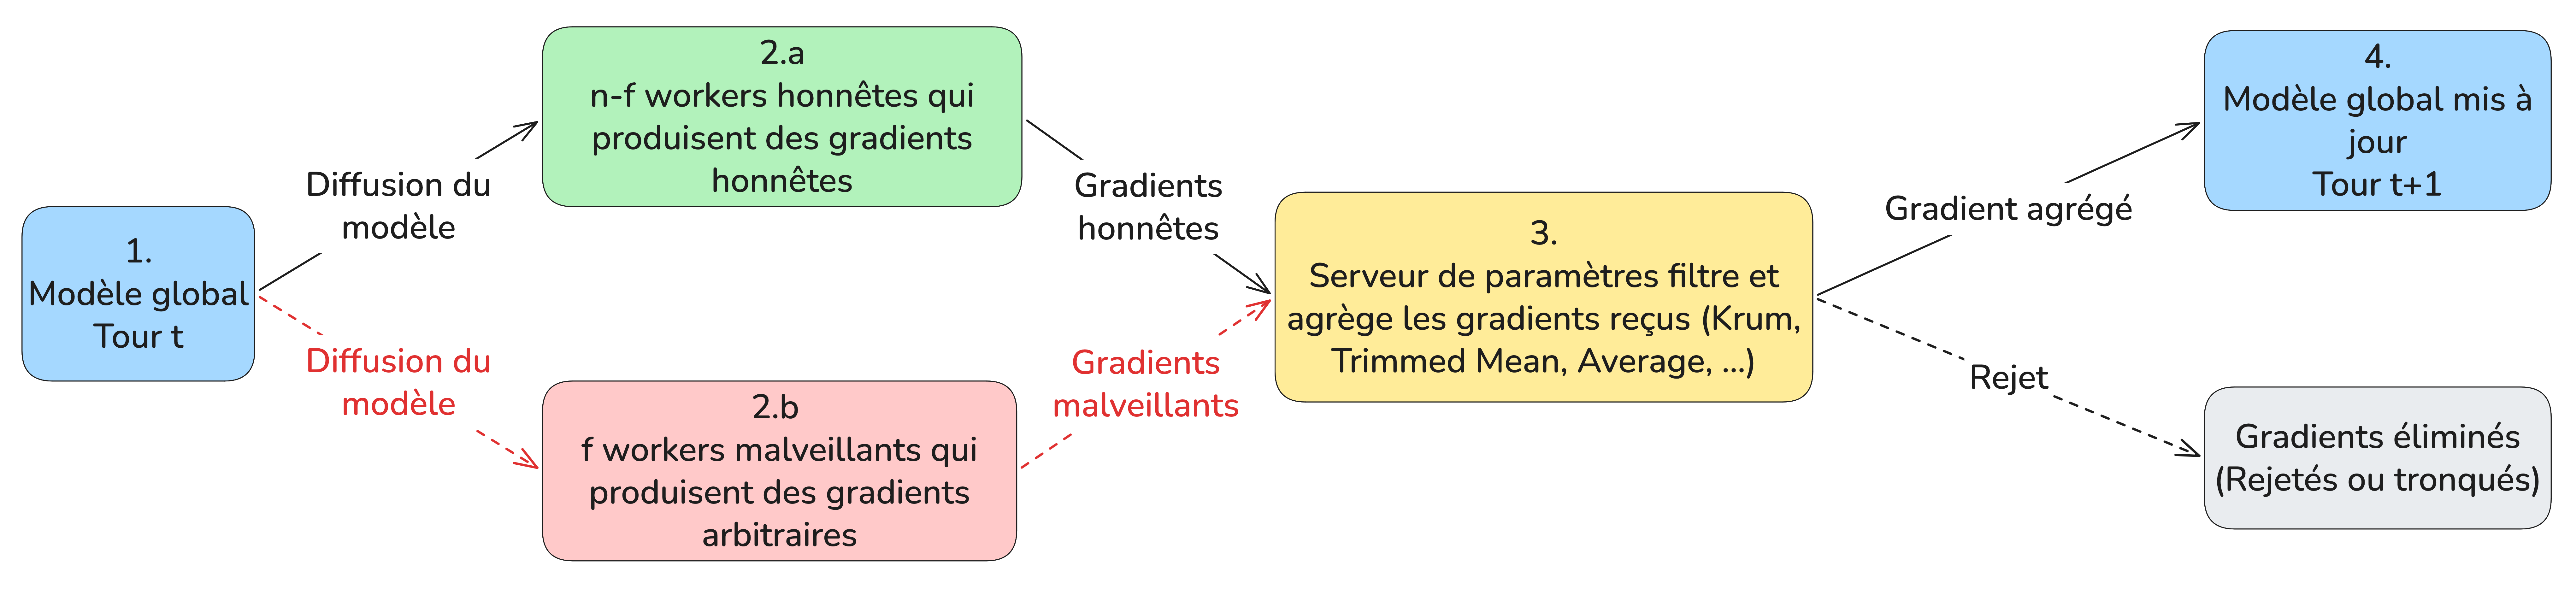
\includegraphics[width=\textwidth]{app-federe-byzantin-centralise.png}
        \par}

    \medskip
    La \textbf{descente de gradient stochastique} (SGD) estime le gradient
    sur un \textbf{mini-lot} d'exemples locaux, puis met à jour le modèle
    dans la direction opposée à ce gradient.

    \medskip
    En \textbf{décentralisé}, les participants mettent à jour leurs modèles
    par des échanges entre voisins, sans serveur central.
\end{frame}

% MIN 4:15 à 5:30. Situer les trois surfaces d'attaque et délimiter le sujet.
\begin{frame}{Des participants malhonnêtes}
    \textbf{Trois surfaces d'attaque}

    \begin{columns}[T]
        \begin{column}{0.30\textwidth}
            \textit{Les données}\\
            L'attaquant altère les exemples.
        \end{column}
        \begin{column}{0.30\textwidth}
            \textit{Le serveur}\\
            L'attaquant compromet le point central.
        \end{column}
        \begin{column}{0.34\textwidth}
            \textbf{Les gradients envoyés}\\
            Des workers malhonnêtes forgent leurs contributions.
        \end{column}
    \end{columns}

    \medskip
    Nous étudions les \textbf{gradients forgés}.
    Dans le \textbf{scénario byzantin}, parmi les $\nworkers$ workers,
    au plus $\nbyz$ sont \textbf{malhonnêtes}.
    Ils peuvent envoyer des vecteurs arbitraires.

    \begin{itemize}
        \item \textbf{Collusion} : les attaquants coordonnent leurs vecteurs.
        \item \textbf{Omniscience} : ils connaissent l'état du système,
            dont les gradients honnêtes.
    \end{itemize}

    Le serveur doit agréger ces vecteurs sans savoir lesquels viennent de
    participants malhonnêtes.
\end{frame}

% MIN 5:30 à 6:30. Montrer l'échec de la moyenne et faire le pont statistique.
\begin{frame}{Pourquoi remplacer la moyenne ?}
    Un attaquant peut déplacer la moyenne aussi loin qu'il le souhaite en
    envoyant un vecteur de grande amplitude dans la direction de son choix.

    Blanchard et al., NeurIPS 2017, lemme 1.

    \begin{block}{Agrégation robuste}
        La règle doit limiter l'influence des attaquants tout en fournissant
        une direction utile à chaque tour d'optimisation.
    \end{block}
\end{frame}

% MIN 6:30 à 7:15. Partir du constat de Sébastien avant d'énoncer la mission.
\begin{frame}{Du copier-coller à des composants réutilisables}
    Des chercheurs reprenaient le code de Sébastien par copier-coller, sans
    toujours le comprendre.

    Mon audit initial et mes reproductions centralisées de zéro m'ont confronté
    à ces difficultés.

    \begin{block}{La mission initiale du stage}
        Réunir les outils nécessaires pour reproduire et comparer ces expériences.
    \end{block}
\end{frame}

% MIN 7:15 à 8:00. Préciser mon périmètre, puis annoncer les trois couches.
\begin{frame}{Krum : une bibliothèque en trois couches}
    Krum est une bibliothèque Python fondée sur \textbf{PyTorch}, un outil
    de calcul et d'entraînement des modèles.

    \begin{tabular}{@{}ll@{}}
        \textbf{Primitives} & Briques de calcul.\\[0.3em]
        \textbf{Simulations} & Exécution des protocoles.\\[0.3em]
        \textbf{Orchestration} & Gestion des campagnes d'expériences.
    \end{tabular}

    \begin{block}{Mes contributions dans ce projet collectif}
        J'ai développé des agrégateurs et travaillé sur le composant \code{Model},
        les architectures de modèles et les simulations centralisés. Le composant \code{Model}
        donne accès aux paramètres sans les recopier.

        J'ai aussi entièrement rédigé la documentation et les tutoriels.
    \end{block}

    \medskip
    Sébastien Rouault et Peva Blanchard ont développé l'orchestrateur.
\end{frame}

\section{Primitives}
% Les primitives constituent les briques de calcul de la bibliothèque.
% Les contributions personnelles sont précisées dans content/03-mission.tex.

\subsection{Agrégateurs}

% MIN 8:00 à 9:00. Présenter les mécanismes et la moyenne de référence.
\begin{frame}{Les familles d'agrégateurs}
    J'ai pris en charge leur implémentation et leurs tests.

    \medskip
    \begin{tabular}{@{}p{0.24\textwidth}p{0.72\textwidth}@{}}
        \textbf{Distances} & Sélection de gradients proches. \\[0.35em]
        \textbf{Coordonnées} & Filtrage de chaque coordonnée séparément. \\[0.35em]
        \textbf{Hybrides} & Combinaison de sélection et de filtrage. \\[0.35em]
        \textbf{Géométrie} & Recherche d'un centre des vecteurs.
    \end{tabular}

    \begin{block}{La moyenne comme référence : \average{}}
        Pour les gradients reçus $\vect{g}_1,\ldots,\vect{g}_{\nworkers}$,
        \[
            \operatorname{Average}=\frac{1}{\nworkers}
            \sum_{i=1}^{\nworkers}\vect{g}_i.
        \]
        La moyenne inclut toutes les contributions, même arbitraires.
    \end{block}
    % À l'oral, rappeler l'appui sur les règles publiées et le code de Sébastien.
\end{frame}

% MIN 9:00 à 10:35. Lire le score, puis la moyenne de la variante implémentée.
% L'annexe du rapport précise l'écart avec la construction itérative publiée.
\begin{frame}{\mkrum{} : sélectionner puis moyenner}
    Au plus $\nbyz$ des $\nworkers$ participants sont \textbf{malhonnêtes}.

    \medskip
    $\mathcal N_i$ contient les $\nworkers-\nbyz-2$ plus proches voisins
    de $\vect{g}_i$ parmi les \textbf{autres} gradients.
    \[
        s_i=\sum_{j\in\mathcal N_i}
        \norm{\vect{g}_i-\vect{g}_j}^{2}.
    \]
    On calcule les scores une seule fois. $I_{\nselected}$ contient les indices
    des $\nselected$ gradients ayant les scores les plus faibles.
    \[
        \operatorname{MultiKrum}(\vect{g}_1,\ldots,\vect{g}_{\nworkers})
        =\frac{1}{\nselected}\sum_{i\in I_{\nselected}}\vect{g}_i.
    \]
    Pour $\nselected=1$, on retrouve \textbf{\krum{}}.
    Pour $\nselected=n$, on retrouve \textbf{Average}.
\end{frame}

\subsection{Attaques}

% MIN 10:35 à 11:25. Expliquer les deux attaques utilisées dans les résultats.
\begin{frame}{Deux attaques pour éprouver les agrégateurs}
    \alert{\textbf{Rappel : scénario d'omniscience.}}\\
    Les attaquants ont accès aux gradients honnêtes.

    \medskip
    On note $\bar{\vect{g}}$ la moyenne des gradients honnêtes.
    \begin{columns}[T,onlytextwidth]
        \begin{column}{0.47\textwidth}
            \begin{block}{\signflip{}}
                L'attaque inverse et amplifie la moyenne des gradients honnêtes.
                \[
                    \vect{b}=-\lambda\bar{\vect{g}},\qquad\lambda>0.
                \]
                Tous les participants malhonnêtes envoient ce même vecteur.
            \end{block}
        \end{column}
        \begin{column}{0.49\textwidth}
            \begin{block}{\smallperturbation{}}
                L'attaque décale une seule coordonnée de la moyenne honnête.
                \[
                    \vect{b}=\bar{\vect{g}}+\gamma\vect{e}_k.
                \]
                $\vect{e}_k$ est le vecteur de base de la coordonnée $k$.
                Le vecteur cherche à rester sélectionnable.
            \end{block}
        \end{column}
    \end{columns}
    % La coordonnée de SmallPerturbation a la plus forte variance honnête.
    % L'expérience de 2018 utilise une amplitude fixée, présentée avec ses réglages.
\end{frame}

\subsection{Partitionnement des données}

% MIN 11:25 à 12:10. Distinguer hétérogénéité honnête et attaque.
\begin{frame}{Les données locales peuvent aussi différer}
    \begin{columns}[T,onlytextwidth]
        \begin{column}{0.47\textwidth}
            \begin{block}{Données IID}
                Observations indépendantes et de même loi.

                \smallskip
                Répartition aléatoire en sous-jeux comparables.
            \end{block}
        \end{column}
        \begin{column}{0.49\textwidth}
            \begin{block}{Données non IID}
                Les lois locales peuvent différer.

                \smallskip
                Exemple : les hôpitaux accueillent des populations différentes.
            \end{block}
        \end{column}
    \end{columns}
    \begin{block}{Partitionneurs}
        Distribuer les données entre participants et régler leur hétérogénéité
        pour comparer les agrégateurs.
    \end{block}
    \alert{Même sans attaque, les gradients honnêtes peuvent différer.}
\end{frame}

\subsection{Extension des primitives}

% MIN 12:10 à 12:55. Montrer comment ajouter une primitive réutilisable.
\begin{frame}{Une seule méthode pour ajouter une règle}
    Une méthode est une fonction associée à un composant logiciel.

    \medskip
    \begin{tabular}{@{}ll@{}}
        \textbf{Primitive} & \textbf{Méthode à implémenter} \\[0.4em]
        Agrégateur & \code{aggregate} \\[0.3em]
        Attaque & \code{generate} \\[0.3em]
        Partitionneur & \code{partition}
    \end{tabular}

    L'interface commune permet de réutiliser la primitive dans les simulations
    sans réécrire leur boucle.

    \medskip
    Au total, la bibliothèque comprend onze règles, cinq attaques,
    quatre partitionneurs et six architectures de modèles.
\end{frame}

\subsection{Modèles pour l'agrégation}

% MIN 12:55 à 15:00. Expliquer le rôle du composant sans détailler l'implémentation.
% Le dessin utilise picture et les couleurs Beamer, sans dépendance supplémentaire.
\begin{frame}{Préparer les modèles pour l'agrégation}
    PyTorch stocke les paramètres et les gradients par couche.
    Pour les agréger, le composant \code{Model} les présente sous forme
    d'une suite de valeurs.

    \begin{center}
        \begingroup
        \setlength{\unitlength}{1mm}
        \setlength{\fboxsep}{0pt}
        \begin{picture}(112,33)
            \put(0,25){\makebox(39,6)[l]{Valeurs par couche}}
            \put(42,23){\colorbox{structure.fg!15}{\makebox(44,10){$\begin{matrix}a&b\\c&d\end{matrix}$}}}
            \put(86,23){\colorbox{defenseAccent!20}{\makebox(22,10){$[\,e\quad f\,]$}}}
            \put(64,22){\vector(0,-1){5}}
            \put(64,17){\vector(0,1){5}}
            \put(97,22){\vector(0,-1){5}}
            \put(97,17){\vector(0,1){5}}
            \put(0,10){\makebox(39,6)[l]{Valeurs réunies}}
            \put(42,10){\colorbox{structure.fg!15}{\makebox(11,6){$a$}}}
            \put(53,10){\colorbox{structure.fg!15}{\makebox(11,6){$b$}}}
            \put(64,10){\colorbox{structure.fg!15}{\makebox(11,6){$c$}}}
            \put(75,10){\colorbox{structure.fg!15}{\makebox(11,6){$d$}}}
            \put(86,10){\colorbox{defenseAccent!20}{\makebox(11,6){$e$}}}
            \put(97,10){\colorbox{defenseAccent!20}{\makebox(11,6){$f$}}}
            \put(42,7){\line(1,0){66}}
            \put(42,7){\line(0,1){2}}
            \put(108,7){\line(0,1){2}}
            \put(42,0){\makebox(66,4){Même mémoire}}
        \end{picture}
        \endgroup
    \end{center}
    La vue réunie partage la mémoire avec les valeurs par couche, ce qui évite
    de les recopier pour l'agrégateur. Le calcul des gradients reste nécessaire.
    % Le même principe s'applique aux paramètres et aux gradients.
    % Le schéma représente l'un de ces ensembles, avec son propre bloc de mémoire.
    % Une concaténation naïve recopierait le vecteur à chaque accès.
\end{frame}

\section{Simulations}
% MIN 15:00 à 16:00. Partir des reproductions menées de zéro.
\begin{frame}{La simulation prend en charge la boucle d'entraînement}
    En reproduisant des expériences à partir de zéro, j'ai dû réécrire
    la même boucle d'entraînement.

    \medskip
    \textbf{L'utilisateur} choisit la répartition des données entre participants.

    \begin{block}{La simulation automatise le protocole}
        \begin{enumerate}
            \item Former et tirer les petits lots de données.
            \item Calculer les gradients locaux.
            \item Appliquer l'attaque et l'agrégation.
            \item Mettre à jour le modèle.
        \end{enumerate}
    \end{block}
\end{frame}

% MIN 16:00 à 17:00. Définir la fidélité d'une simulation.
\begin{frame}{Fidélité des simulations}
    \begin{block}{L'objectif}
        La simulation permet de faire varier les paramètres de l'expérience tout en gardant
        la même boucle d'entraînement sous PyTorch.
    \end{block}
    \medskip
    \begin{block}{Fidélité au protocole}
        Une simulation fidèle conserve les mécanismes du protocole nécessaires
        à l'étude du phénomène visé et documente les adaptations apportées.
    \end{block}
\end{frame}

\section{Orchestration}
% MIN 17:00 à 17:45. Expliquer les services, sans détailler les fonctions internes.
\begin{frame}{L'orchestrateur gère les campagnes}
    L'orchestrateur lance les combinaisons de paramètres et enregistre les résultats.

    À la relance, il ne reprend que les expériences nouvelles, échouées ou périmées.

    \medskip
    Développé par Sébastien Rouault et Peva Blanchard.
    % La relance concerne une expérience entière.
    % Elle ne promet pas une reprise au dernier tour d'entraînement.
\end{frame}

\section{Qualité logicielle}
% MIN 17:45 à 19:00. Présenter les tests, la documentation et l'installation.
\begin{frame}{Qualité et distribution de la bibliothèque}
    \begin{itemize}
        \item Plusieurs centaines de tests automatisés vérifient le comportement
              des composants.
        \item J'ai entièrement rédigé la documentation et les tutoriels pour
              expliquer comment utiliser et étendre la bibliothèque.
    \end{itemize}

    \medskip
    \begin{center}
        Licence MIT\hspace{1.5em}\code{pip install krum}
    \end{center}
\end{frame}

\section{Expériences}
% ================= VALIDATION EXPÉRIMENTALE =================
% Deux expériences centralisées. Les durées comprennent la lecture des figures.

% MIN 19:00 à 20:00. Poser la question et signaler le réglage hors garantie.
\begin{frame}{2017 : \mkrum{} face à la moyenne}
    \textbf{La sélection maintient-elle l'apprentissage sous attaque ?}
    \medskip
    \begin{columns}[T,onlytextwidth]
        \begin{column}{0.47\textwidth}
            \textbf{Données et modèle}
            \par Spambase : courriels, 57 variables, deux catégories.
            \par Deux couches cachées de 20 neurones.
        \end{column}
        \begin{column}{0.49\textwidth}
            \textbf{Scénario byzantin}
            \par 20 workers, dont 6 malhonnêtes.
            \par \signflip{} inverse la moyenne des gradients honnêtes et l'amplifie par 10.
        \end{column}
    \end{columns}
    \medskip
    Données indépendantes et de même loi (IID).\\
    300 tours. Pas $0{,}01$. Graine 42.
    \begin{block}{Un réglage hors garantie}
        Sous attaque : $\nselected=\nworkers-\nbyz=14$.
        \par Sans attaque : $\nselected=\nworkers$, donc \mkrum{} coïncide avec la moyenne.
    \end{block}
    {\small Légendes : \textcode{Mean} désigne \average{} ; \textcode{f0} et \textcode{f6} indiquent 0 et 6 malhonnêtes.\par}
    {\footnotesize Blanchard et al., NeurIPS 2017. Protocole adapté, observation hors garantie.\par}
\end{frame}

% MIN 20:00 à 21:00. Lire l'augmentation de la perte de la moyenne attaquée.
\begin{frame}[t]{2017 : la perte de la moyenne diverge}
    \setlength{\parskip}{0pt}
    \begin{columns}[c,onlytextwidth]
        \begin{column}{0.50\textwidth}
            % Le PNG mesure 1600 par 956 pixels à 100 dpi, soit 0,72 bp par pixel.
            % Le panneau de perte test conserve x de 132 à 760 et y de 80 à 360.
            \includegraphics[width=\linewidth,
                trim={95.04bp 429.12bp 604.8bp 57.6bp}, clip]{"Krum NeurIPS 2017.png"}
        \end{column}
        \begin{column}{0.46\textwidth}
            \textbf{Moyenne attaquée}\\
            À partir du tour 40, les poids deviennent indéfinis (NaN).
            \par\medskip
            \alert{Les 60\,\% reflètent la classe majoritaire.}\\
            Le modèle n'a plus de performance valide.
        \end{column}
    \end{columns}
    \par\smallskip
    % Le panneau d'exactitude test est conservé en entier avec ses axes et sa légende.
    % Son rectangle va de x=130 à x=1450 et de y=630 à y=906.
    {\centering
        \includegraphics[width=0.95\textwidth,
            trim={93.6bp 36bp 108bp 453.6bp}, clip]{"Krum NeurIPS 2017.png"}
        \par}
    {\footnotesize Blanchard et al., NeurIPS 2017. Perte test en haut, exactitude test en bas.\par}
\end{frame}

% MIN 21:00 à 22:00. Comparer les pertes finies et borner la conclusion.
\begin{frame}[t]{2017 : \mkrum{} continue à apprendre}
    \setlength{\parskip}{0pt}
    \begin{columns}[c,onlytextwidth]
        \begin{column}{0.50\textwidth}
            % Le panneau supérieur droit exclut déjà la moyenne attaquée.
            % Le rectangle conserve x de 828 à 1448 et y de 80 à 360.
            \includegraphics[width=\linewidth,
                trim={596.16bp 429.12bp 109.44bp 57.6bp}, clip]{"Krum NeurIPS 2017.png"}
        \end{column}
        \begin{column}{0.46\textwidth}
            \textbf{Zoom de $0{,}4$ à $0{,}8$.}\\
            La moyenne attaquée est exclue.\\
            \par\medskip
            Exactitude : environ \textbf{77\,\% sous attaque}, contre \textbf{82\,\% sans attaque}.
            \par\smallskip
            $\nselected=14$, hors garantie.
        \end{column}
    \end{columns}
    \par\smallskip
    % Le même panneau complet d'exactitude garde toutes les courbes et sa légende.
    {\centering
        \includegraphics[width=0.95\textwidth,
            trim={93.6bp 36bp 108bp 453.6bp}, clip]{"Krum NeurIPS 2017.png"}
        \par}
    {\footnotesize Blanchard et al., NeurIPS 2017. Perte test en haut, exactitude test en bas.\par}
\end{frame}

% MIN 22:00 à 23:20. Expliquer l'attaque ciblée et les deux filtres de Bulyan.
% Le modèle est un réseau avec une couche cachée de 100 neurones.
% La variante documentée de Bulyan sélectionne n-2f-2 vecteurs, au lieu de n-2f.
% MultiKrum calcule ses scores en une passe. Ici, m=1 désigne bien Krum.
\begin{frame}{2018 : une perturbation peut passer la sélection}
    \textbf{Un gradient proche des honnêtes peut-il dégrader \krum{} ?}
    \medskip
    \begin{columns}[T,onlytextwidth]
        \begin{column}{0.47\textwidth}
            \textbf{Données et modèle}
            \par MNIST : images de chiffres manuscrits.
            \par Une couche cachée de 100 neurones.
        \end{column}
        \begin{column}{0.49\textwidth}
            \textbf{Scénario byzantin}
            \par 39 workers, dont 9 malhonnêtes.
            \par \smallperturbation{} décale une coordonnée, $\gamma=4$ fixé.
            \par Le vecteur reste sélectionné à chaque tour.
        \end{column}
    \end{columns}
    \smallskip
    Données IID. 300 tours. Graine 42.\\
    \mkrum{} avec $\nselected=1$ est \krum{} ; \bulyan{} subit la même attaque.
    \begin{block}{\bulyan{} ajoute un second filtre}
        \begin{enumerate}
            \item Sélection de vecteurs selon leurs distances.
            \item Pour chaque coordonnée, moyenne des valeurs les plus proches de la médiane.
        \end{enumerate}
    \end{block}
    {\footnotesize El-Mhamdi et al., ICML 2018. Protocole adapté.\par}
\end{frame}

% MIN 23:20 à 25:00. Lire le plateau et comparer à la référence sans attaque.
\begin{frame}{2018 : \krum{} apprend, puis plafonne}
    \setlength{\parskip}{0pt}
    \centering
    % Cadrages des panneaux perte test et exactitude du PNG de 2250 par 600 pixels.
    % La résolution est d'environ 150 dpi, soit 0,48 bp par pixel.
    % Le panneau central de perte d'entraînement est omis pour agrandir les deux autres.
    % Les deux panneaux gardent tous leurs axes, légendes et courbes, sans déformation.
    % Rectangles conservés : x de 20 à 745 et de 1515 à 2235, y de 60 à 580.
    \includegraphics[width=0.44\textwidth,
        trim={9.6bp 9.6bp 722.4bp 28.8bp}, clip]{"Hidden Vulnerability ICML 2018.png"}
    \hfill
    \includegraphics[width=0.44\textwidth,
        trim={727.2bp 9.6bp 7.2bp 28.8bp}, clip]{"Hidden Vulnerability ICML 2018.png"}
    \par\smallskip
    \begin{tabular}{ccc}
        \krum{} attaqué & \bulyan{} attaqué & Moyenne sans attaque \\
        $\approx\mathbf{90\,\%}$ & $\approx\mathbf{94\,\%}$ & $\approx\mathbf{95\,\%}$
    \end{tabular}
    \par\medskip
    {\small La perturbation passe la sélection de \krum{} à chaque tour et dégrade peu à peu le résultat.\par}
    \par\smallskip
    {\footnotesize Exactitude finale. El-Mhamdi et al., ICML 2018.\par}
\end{frame}

% MIN 25:00 à 25:30. Distinguer fidélité, répétabilité et portée empirique.
\begin{frame}{Ce que ces expériences permettent de conclure}
    Les expériences retrouvent les phénomènes visés, avec des adaptations
    documentées.
    \par\medskip
    À code, graines, matériel et environnement déterministe fixés, deux
    exécutions donnent les mêmes résultats bit à bit.
    \par\medskip
    Moins de trois minutes par expérience sur CPU, le processeur de la machine.
    \par\medskip
    L'équipe a aussi implémenté \monna{}, un protocole décentralisé
    (Farhadkhani et al., ICML 2023).
\end{frame}

\section{Positionnement et limites}
% La comparaison situe la bibliothèque et ses limites.

% MIN 25:30 à 26:30. Comparaison des bibliothèques retenues pour le rapport.
\begin{frame}{Face à cinq bibliothèques comparables}
    Pour la comparaison, j'ai retenu ByzFL, FedLab, Blades,
    FL-Byzantine-Library et ByzPy, dont les composants d'agrégation byzantine
    sont ouverts et comparables.

    \medskip
    {\renewcommand{\arraystretch}{1.2}
    \begin{tabular}{@{}p{0.18\textwidth}p{0.34\textwidth}p{0.40\textwidth}@{}}
        \textbf{Critère} & \textbf{Krum} & \textbf{Dans la comparaison} \\
        \hline
        Catalogue & 11 règles et 5 attaques. & Certaines bibliothèques proposent plus de composants. \\
        Zéro-copie & \code{Model} partage la mémoire. & L'accès copie les valeurs ou n'a pas d'équivalent. \\
        Protocoles & Trois protocoles documentés. & Cadres génériques ou suites. \\
        Relance & Recalcul des résultats périmés. & ByzFL saute les exécutions terminées.
    \end{tabular}}

    \medskip
    J'ai analysé ces composants.\\
    {\small Comptes d'août 2026, audités en septembre 2026.}
\end{frame}

% MIN 26:30 à 27:00. Limites du catalogue et des conditions d'exécution.
\begin{frame}{Les limites actuelles}
    \begin{itemize}
        \item Le catalogue reste ciblé. Certaines bibliothèques proposent plus de composants.
        \item Les pré-agrégateurs ne sont pas inclus. Appliqués avant l'agrégation,
              ils peuvent borner les normes ou réduire le bruit.
        \item Les expériences s'exécutent séquentiellement sur une seule machine.
              Les échanges entre participants sont simulés. On évalue donc les
              protocoles, pas un déploiement distribué réel.
    \end{itemize}
\end{frame}

\section{Bilan et perspectives}
% MIN 27:00 à 28:00. Contributions personnelles, papier compagnon et acquis.
\begin{frame}{Mes contributions au projet}
    Mon travail a porté sur les agrégateurs, \code{Model}, les architectures de modèles et les
    simulations centralisés. J'ai écrit les tests associés automatisés.

    J'ai aussi entièrement rédigé la documentation et les tutoriels. J'ai
    assuré une partie de la rédaction du papier compagnon, puis l'ai corrigé
    avec El-Mahdi El-Mhamdi.

    \smallskip
    {\small Le papier est en cours de rédaction. Il vise la rubrique logiciels
    libres du \textit{Journal of Machine Learning Research} (JMLR).}

    \medskip
    Le stage m'a appris à justifier mes décisions d'architectures et à faire relire mon code.
    J'ai commencé à apprendre à lire des articles de recherche. J'ai aussi
    découvert la rédaction d'un article scientifique.
\end{frame}

% MIN 28:00 à 29:00. Bilan des travaux, bénéfices ISF et prolongement en thèse.
\begin{frame}{Les acquis du stage et la suite}
    Krum réunit des composants réutilisables pour reproduire et comparer
    des expériences d'agrégation robuste.

    \bigskip
    \begin{columns}[T,onlytextwidth]
        \begin{column}{0.47\textwidth}
            \begin{block}{Les acquis ISF en pratique}
                J'ai relié statistiques et optimisation au code testé,
                puis à l'analyse des résultats.

                Le travail en équipe m'a appris à expliquer et documenter mes choix.
            \end{block}
        \end{column}
        \begin{column}{0.47\textwidth}
            \begin{block}{La thèse dans la chaire ATLAS}
                J'étudierai les garanties des agrégateurs pour la sécurité de l'apprentissage.

                Krum servira à mener des campagnes expérimentales comparables.
            \end{block}
        \end{column}
    \end{columns}

    \bigskip
    \centering
    Merci à l'équipe et merci de votre attention.
\end{frame}

% MIN 29:00 à 30:00. Cette minute reste une marge pour l'exposé principal.

\appendix

% Séparation blanche entre l'exposé et les slides de réserve.
\begin{frame}[plain,noframenumbering]
\end{frame}

% RÉSERVE. Étude collective MoNNA, hors du périmètre personnel d'Arthur.
\begin{frame}{\monna{} décentralisé : étude de cas ICML 2023}
    \small
    L'équipe a réalisé cette simulation et analysé ses résultats.
    Mon travail portait sur le cas centralisé.

    MNIST réduit : $n=16$, $f=5$, 200 tours, \signflip{} d'amplitude 1.

    {\centering
        \includegraphics[width=\textwidth]{"MoNNA ICML 2023.png"}
        \par}

    La règle \nna{} moyenne les modèles les plus proches du modèle local.\\
    Exactitude finale sous attaque : \nna{} $\approx84\,\%$,
    \average{} $\approx10\,\%$. Sans attaque : $\approx87\,\%$.

    Farhadkhani et al., ICML 2023.
\end{frame}

% RÉSERVE. Extraits du listing de l'annexe 08 du mémoire.
\begin{frame}[fragile]{Une expérience centralisée}
    \small
    \begin{verbatim}
sim = KrumSimulation(
    model_cls=Krum2017MLPMnist,
    train_datasets=worker_datasets, test_set=test_set,
    aggregator=aggregator, attack=attack,
    n=n, f=f, rounds=100, batch_size=32, lr=0.1, seed=seed,
)
sim.setup()

loss = Metric("loss", dtype=float)
accuracy = Metric("accuracy", dtype=float)
for step in range(100):
    sim.step()
    if step % 10 == 0:
        test_loss, test_accuracy = sim.evaluate()
        loss.push(step, test_loss, skip_if_exists=True)
        accuracy.push(step, test_accuracy, skip_if_exists=True)
    \end{verbatim}

    La fonction d'évaluation calcule la perte et l'exactitude,
    c'est-à-dire la proportion de prédictions correctes.

    \medskip
    {\footnotesize Extrait du listing de l'annexe 08.}
\end{frame}

% RÉSERVE. Balayage de configurations tiré du listing de l'annexe 08.
\begin{frame}[fragile]{Faire varier les configurations d'une campagne}
    \small
    \begin{verbatim}
with Orchestrator("krum_byzantine_study") as orch:
    for n, f in [(13, 2), (25, 5)]:
        for aggregator in [Average, Krum, Bulyan]:
            for attack in [ALIEAttack, SignFlipAttack, None]:
                orch.run(
                    experiment, n=n, f=f,
                    aggregator=aggregator, attack=attack, seed=42,
                )

loss_df = orch.get("loss").to_pandas()
acc_df = orch.get("accuracy").to_pandas()
    \end{verbatim}

    \code{None} signifie qu'aucune attaque n'est appliquée.
    Les mesures sont converties en tableaux avec la bibliothèque pandas.
    L'orchestrateur a été développé par Sébastien Rouault et Peva Blanchard.

    \medskip
    {\footnotesize Extrait du listing de l'annexe 08.}
\end{frame}

% RÉSERVE. Notations des onze règles d'agrégation implémentées.
\begin{frame}{Notations des agrégateurs : moyenne et coordonnées}
    \small
    Soient $\vect{x}_1,\ldots,\vect{x}_n\in\mathbb{R}^d$ les gradients reçus.
    Pour une coordonnée $k$, $x_{(1),k}\leq\cdots\leq x_{(n),k}$ désigne
    les valeurs triées.

    \begin{align*}
        \texttt{Average}:\quad
        & A=\frac{1}{n}\sum_{i=1}^{n}\vect{x}_i.
        \\
        \texttt{Median}:\quad
        & M_k=\operatorname{med}_{i=1,\ldots,n}x_{i,k}.
        \\
        \texttt{TrimmedMean}:\quad
        & T_k=\frac{1}{n-2f}\sum_{r=f+1}^{n-f}x_{(r),k}.
    \end{align*}
    \texttt{TrimmedMean} retire donc les $f$ valeurs extrêmes de chaque côté,
    séparément pour chaque coordonnée.
\end{frame}

% RÉSERVE. Krum, MultiKrum et Bulyan.
\begin{frame}{Notations des agrégateurs : distances et filtrage}
    \small
    Pour chaque $i$, $\mathcal{N}_i$ contient les $n-f-2$ gradients les plus
    proches de $\vect{x}_i$ parmi les autres gradients.
    \[
        s_i=\sum_{j\in\mathcal{N}_i}\norm{\vect{x}_i-\vect{x}_j}^{2},
        \qquad i^*=\arg\min_i s_i.
    \]
    \begin{align*}
        \texttt{Krum}:\quad & \vect{x}_{i^*}.
        \\
        \texttt{MultiKrum}:\quad
        & \frac{1}{m}\sum_{i\in I_m}\vect{x}_i,
          \quad I_m=\text{indices des $m$ plus petits scores }s_i.
    \end{align*}
    Les scores sont calculés une seule fois dans la bibliothèque.

    \medskip
    \texttt{Bulyan} sélectionne itérativement $\theta=n-2f-2$ candidats avec
    \texttt{MultiKrum}. Pour chaque coordonnée $k$, il moyenne les
    $\theta-2f$ valeurs sélectionnées les plus proches de leur médiane.
    \[
        B_k=\frac{1}{\theta-2f}\sum_{r\in J_k}x_{(r),k},
        \qquad |J_k|=\theta-2f.
    \]
\end{frame}

% RÉSERVE. Méthodes géométriques et énumératives.
\begin{frame}{Notations des agrégateurs : géométrie et recherche}
    \small
    \begin{align*}
        \texttt{GeoMed}:\quad
        & \arg\min_{\vect{y}\in\mathbb{R}^d}
          \sum_{i=1}^{n}\norm{\vect{y}-\vect{x}_i}.
        \\
        \texttt{Medoid}:\quad
        & \arg\min_{\vect{x}\in\{\vect{x}_1,\ldots,\vect{x}_n\}}
          \sum_{i=1}^{n}\norm{\vect{x}-\vect{x}_i}.
        \\
        \texttt{Brute}:\quad
        & \frac{1}{|S^*|}\sum_{i\in S^*}\vect{x}_i,
          \quad S^*=\arg\min_{\substack{S\subseteq\{1,\ldots,n\}\\|S|=n-f}}
          \max_{i,j\in S}\norm{\vect{x}_i-\vect{x}_j}.
    \end{align*}
    \texttt{GeoMed} minimise la somme des distances sans imposer que la sortie
    soit un gradient reçu. \texttt{Medoid} impose cette contrainte.
    \texttt{Brute} choisit le sous-ensemble de diamètre minimal.
\end{frame}

% RÉSERVE. AKSEL et NNA.
\begin{frame}{Notations des agrégateurs : pivot et voisinage}
    \small
    \texttt{AKSEL} prend pour pivot $\vect{p}$ la médiane coordonnée par
    coordonnée, puis moyenne les $n-f$ gradients les plus proches de ce pivot.
    \[
        p_k=\operatorname{med}_{i=1,\ldots,n}x_{i,k},
        \qquad
        \operatorname{AKSEL}(\vect{x}_{1:n})=
        \frac{1}{n-f}\sum_{i\in I_{n-f}}\vect{x}_i,
        \quad I_{n-f}=\text{indices les plus proches de }\vect{p}.
    \]

    \medskip
    Pour \texttt{NNA}, $\vect{z}^{(0)}$ est le pivot et $q$ est le nombre
    de vecteurs à agréger, paramètre \texttt{num\_closest}. L'application
    $\tau$ ordonne les autres vecteurs reçus par distance croissante au pivot,
    de sorte que
    la sortie inclut le pivot et ses $q-1$ plus proches voisins :
    \[
        \operatorname{NNA}=\frac{1}{q}\sum_{r=0}^{q-1}
        \vect{z}^{(\tau(r))},
        \qquad \tau(0)=0.
    \]
    Dans \texttt{MoNNA}, le modèle local sert de pivot et $q=n-2f$.
\end{frame}

% RÉSERVE. Notations des cinq attaques implémentées.
\begin{frame}{Notations des attaques : gradients honnêtes et statistiques}
    \small
    On note $\mathcal{H}$ l'ensemble des gradients honnêtes,
    $|\mathcal{H}|=n-f$, et
    $\bar{\vect{g}}=\frac{1}{n-f}\sum_{i\in\mathcal{H}}\vect{g}_i$.
    Pour chaque coordonnée $k$, $\mu_k$ et $\sigma_k$ sont la moyenne et
    l'écart-type honnêtes.

    \begin{align*}
        \texttt{SignFlip}:\quad
        & \vect{b}=-c\,\bar{\vect{g}}.
        \\
        \texttt{ALIE}:\quad
        & b_k=\mu_k\pm z\sigma_k,
          \quad\text{avec le signe choisi pour l'attaque.}
        \\
        \texttt{Gaussian}:\quad
        & \vect{b}\sim\mathcal{N}(\mu_G\vect{1},\sigma_G^2 I_d),
          \quad\text{indépendamment des gradients honnêtes.}
    \end{align*}
    Les $f$ participants malveillants envoient chacun le vecteur ainsi défini.
    Pour \texttt{ALIE}, $z$ règle l'écart aux statistiques honnêtes. Pour
    \texttt{Gaussian}, $\mu_G$ et $\sigma_G$ sont les paramètres du bruit.
\end{frame}

% RÉSERVE. Attaques ciblées de la vulnérabilité cachée.
\begin{frame}{Notations des attaques : négation et perturbation}
    \small
    \texttt{FullGradientNegation} suppose connu le gradient calculé sur
    l'ensemble des données :
    \[
        \vect{b}=-\kappa\vect{g}_{\mathrm{full}}.
    \]

    \medskip
    \texttt{SmallPerturbation} part de la moyenne honnête et la décale dans
    une direction $\vect{e}$. L'attaque choisit le plus grand décalage qui
    reste sélectionné par l'agrégateur ciblé :
    \[
        \vect{b}=B(\gamma_m)=\bar{\vect{g}}+\gamma_m\vect{e},
        \qquad
        \gamma_m=\sup\{\gamma\geq0:
        B(\gamma)\text{ est sélectionné}\}.
    \]
    Par défaut, $\vect{e}$ est le vecteur de base de la coordonnée présentant
    la plus forte variance honnête. Les $f$ attaquants envoient ce même vecteur.
\end{frame}

% RÉSERVE. Définition formelle du modèle de menace et de la résilience.
\begin{frame}{Modèle de menace et résilience}
    \small
    Parmi les $n$ gradients reçus, au plus $f$ peuvent être arbitraires.
    Ils peuvent être coordonnés et dépendre des gradients honnêtes.
    Ces derniers sont supposés indépendants, de même loi, et d'espérance
    $\vect{g}$.

    \medskip
    Une règle $F$ est $(\alpha,f)$-résiliente si son espérance reste orientée
    vers le vrai gradient et si ses fluctuations restent contrôlées :
    \[
        \langle\mathbb{E}[F],\vect{g}\rangle
        \geq (1-\sin\alpha)\norm{\vect{g}}^2>0,
        \qquad 0\leq\alpha<\frac{\pi}{2}.
    \]
    Les moments $\mathbb{E}\norm{F}^{r}$, pour $r=2,3,4$, doivent aussi être
    bornés en fonction des moments des gradients honnêtes.

    \medskip
    Cette propriété ne suffit pas seule à prouver la convergence : le bruit
    honnête et le calendrier du pas d'apprentissage interviennent également.
\end{frame}

% RÉSERVE. Écarts des implémentations documentés dans le mémoire.
\begin{frame}{Écarts entre publication et implémentation}
    \small
    \begin{tabular}{@{}p{0.18\textwidth}p{0.39\textwidth}p{0.37\textwidth}@{}}
        \textbf{Règle} & \textbf{Publication} & \textbf{Bibliothèque} \\
        \hline
        \texttt{MultiKrum} &
        Sélection itérative, avec recalcul après chaque retrait. &
        Scores calculés une fois, puis moyenne des $m$ plus petits. \\
        \texttt{Bulyan} &
        Sélection de $n-2f$ candidats. &
        Sélection de $n-2f-2$ candidats, puis filtrage coordonnée par coordonnée.
    \end{tabular}

    \medskip
    Pour $m=1$, \texttt{MultiKrum} coïncide avec \texttt{Krum}.
    Les résultats des expériences caractérisent les variantes effectivement
    codées. Une garantie théorique ne se transfère pas automatiquement à une
    variante modifiée.
\end{frame}

% RÉSERVE. Résultats et portée des deux expériences centralisées.
\begin{frame}{Ce que montrent les deux expériences}
    \small
    \begin{block}{Spambase, paramètres de 2017}
        $n=20$, $f=6$, \texttt{MultiKrum} avec $m=14$, \texttt{SignFlip}
        d'amplitude 10. La moyenne diverge dans cette simulation ;
        \texttt{MultiKrum} poursuit l'apprentissage.
        Le réglage $m=14$ dépasse la borne théorique $m\leq5$.
    \end{block}
    \begin{block}{MNIST, attaque de 2018}
        $n=39$, $f=9$, $\gamma=4$. L'exactitude plafonne vers 90\,\% pour
        \texttt{Krum}, contre environ 94\,\% pour \texttt{Bulyan} et 95\,\%
        pour la référence saine.
    \end{block}
    Ces courbes illustrent les phénomènes visés dans ces réglages. Elles
    n'établissent ni une garantie théorique ni une stabilité statistique
    sur plusieurs graines.
\end{frame}

% RÉSERVE. Distinction entre fidélité du protocole et répétabilité.
\begin{frame}{Fidélité, répétabilité et portée}
    \small
    \begin{itemize}
        \item \textbf{Fidélité :} conserver les mécanismes utiles du protocole
        étudié et documenter les adaptations de la simulation.
        \item \textbf{Répétabilité :} une graine fixe les tirages pseudo-aléatoires.
        Dans l'environnement déterministe documenté, relancer la même
        configuration donne les mêmes résultats.
        \item \textbf{Limite :} une graine ne mesure pas la variabilité entre
        exécutions. Il faudrait plusieurs graines et une analyse statistique.
        \item \textbf{Périmètre :} les expériences tournent séquentiellement sur
        une machine ; les échanges entre workers sont simulés.
    \end{itemize}
\end{frame}


\end{document}
